
\chapter{Webová aplikace}

\noindent
Tato kapitola popisuje zvolené postupy při psaní webové aplikace (backend a frontend).

Obrázek \ref{fig:structure_back} a obrázek \ref{fig:structure_front} popisují adresářové
struktury backendu a frontendu.
Některé méně důležite adresáře byly vynechány.

\begin{figure} [!htb]
  \begin{itemize}
    \setlength\itemsep{.05em}
    \item \textbf{config} -- konfigurační soubory
    \item \textbf{scripts} -- skripty pro vývoj
    \item \textbf{test\_assets} -- obrázky pro testování rozpoznávání SPZ
    \item \textbf{src} -- zdrojový kód
    \begin{itemize}
      \setlength\itemsep{.05em}
      \item \textbf{apis} -- helper funkce pro komunikaci s externím API pro rozpoznávání SPZ
      \item \textbf{auth} -- autentifikace a autorizace
      \item \textbf{cache} -- implementace mezipaměti
      \item \textbf{db} -- připojení k databázi a nastavení GraphQL serveru Apollo
      \item \textbf{endpoints} -- endpointy (ne GraphQL)
      \item \textbf{types} -- business logika aplikace, definice GraphQL schema, resolverů a mongoose modelů
      \item \textbf{utils} -- datové struktury a ostatní helper funkce i pro testy
    \end{itemize}
  \end{itemize}
  \caption{Adresářová struktura backendu.}
  \label{fig:structure_back}
  \end{figure}
  
\begin{figure}[!htb]
    \begin{itemize}
      \setlength\itemsep{.05em}
      \item \textbf{config} -- konfigurační soubory
      \item \textbf{src/app} -- zdrojový kód
      \begin{itemize}
        \setlength\itemsep{.05em}
        \item \textbf{apis} -- helper funkce pro získávání obrázků z backendu
        \item \textbf{components} -- komponenty uživatelského rozhraní
        \item \textbf{constants} -- GraphQL dotazy, barvy, apod
        \item \textbf{helpers} -- helper funkce
        \item \textbf{images} -- obrázky
        \item \textbf{layouts} -- rozložení obrazovek
        \item \textbf{pages} -- komponenty obrazovek
        \item \textbf{redux} -- definice reducerů a stavů aplikace
        \item \textbf{routes} -- definice cest obrazovek
        \item \textbf{sagas} -- vedlejší efekty Redux akcí
      \end{itemize}
    \end{itemize}
    \caption{Adresářová struktura frontendu.}
    \label{fig:structure_front}
  \end{figure}

\newpage

Některé konfigurovatelné hodnoty jsou brané z proměnných prostředí, mají ale předdefinovanou hodnotu, pokud
konkrétní proměnná prostředí je prázdná.

Nastavení backendu je řešeno knihovnou nconf, která umožňuje kteroukoliv hodnotu upravit
pomocí proměnných prostředí -- stačí jen vzít cestu k hodnotě a každé vnoření nahradit 
dvěma podtržítky.
\citep[][]{nconf}
Například cesta \texttt{\{ mongo: \{ host \} \}} lze přepsat promměnou prostředí s názvem \texttt{mongo\_\_host}.

Seznam všech závislostí je uveden v souborech \textit{package.json} a \textit{package-lock.json}.

\section{Obrazovky}

\noindent
Mějme po příhlášení do webového rozhraní následující obrazovky,
mezi kterými bude uživatel přepínat pomocí hlavního menu.

\subsection{Správa účtu}

\noindent
Tato stránka umožňuje změnu údajů a hesla současně přihlášeného uživatele.

\subsection{Zařízení}

\noindent
Na této stránce je správa zařízení zachycujících snímky SPZ, která lze autentifikovat do systému pomocí
QR kódu. Pokud však zařízení není aktivováno a QR kód vyprší, tak lze vygenerovat nový.
Obrazovka také zobrauje čas posledního kontaktu se zařízením.
Nastavení zařízení obsahuje směr (dovnitř/ven), parametry pro detekci SPZ popsané v podkapitole \ref{reco_params}
a paramatry pro zmenšení snímky popsané v podkapitole \ref{app_resizing}.

Screenshot obrazovky je na obrázku \ref{fig:page_devices}.

\begin{figure} \centering
  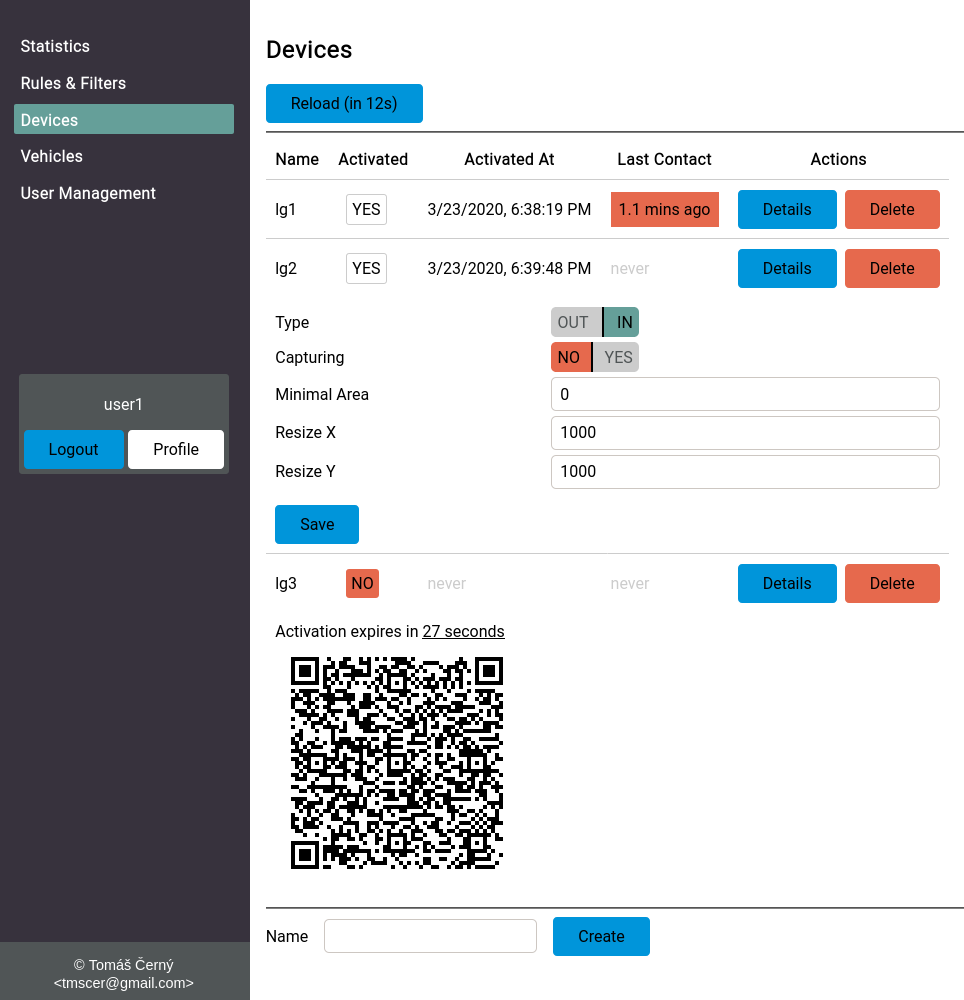
\includegraphics[width=145mm]{../img/page_devices.png}
  \caption[Stránka pro zařízení s hlavním menu.]{Stránka pro zařízení s hlavním menu. Stránka se
  pravidelně aktualizuje. Pokud byl poslední kontakt se zařízením před více jak minutou,
  čas posledního kontaktu se podbarví červeně. Pokud byl poslední kontakt se zařízením
  před více jak hodinou, místo relativního časo se zobrazí čas absolutní.}
  \label{fig:page_devices}
\end{figure}

\subsection{Pravidla a Filtry}

\noindent
Tato stránka umožňuje definici parkovacích pravidel a filtrů vozidel (popsáno v \ref{analysis_parking_schema}).
Pro ověření je možné parkovací pravidla a filtry simulovat.
Obrazovka obsahuje pohled v rámci dne a měsíce.
Je-li potřeba mít ta samá pravidla několik týdnů, měsíců nebo let, lze požadovaný rozsah (týden, měsíc, pár dnů) vybrat
a zkopírovat buď na několik míst, nebo zvolit počáteční datum a počet zkopírování do budoucnosti.

Screenshoty obrazovky jsou na obrázcích \ref{fig:page_rules_filters1}, \ref{fig:page_rules_filters2} a \ref{fig:page_rules_filters3}.

\begin{figure}[htb!] \centering
  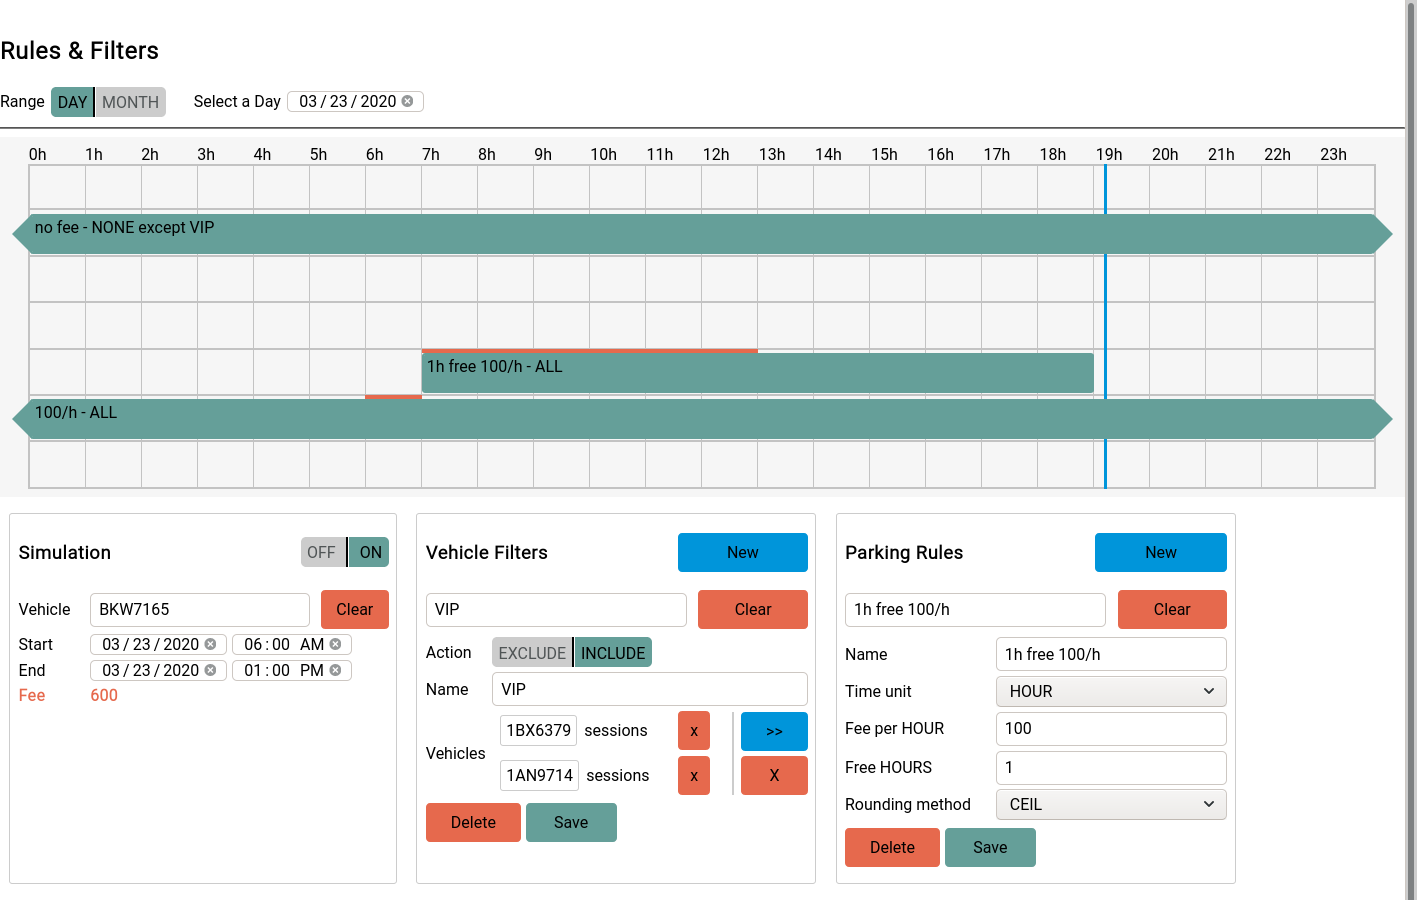
\includegraphics[width=145mm]{../img/page_rules_filters1.png}
  \caption[Stránka s pravidly a filtry -- pohled na jeden den.]{Stránka s pravidly a filtry -- pohled na jeden den.
  Na horizontální ose je čas a na vertikální ose je priorita přiřazení pravidla.
  Kliknutím na blok v kalendáři se otevře editace přiřazení pravidla. Oranžová čára značí simulaci a vlevo
  dole lze spatřit výpočítanou částku k zaplacení. Napravo od panelu se simulací jsou editory definic filtrů
  a pravidel. Modrá horizontální čára značí aktuální čas.}
  \label{fig:page_rules_filters1}
\end{figure}

\begin{figure}[htb!] \centering
  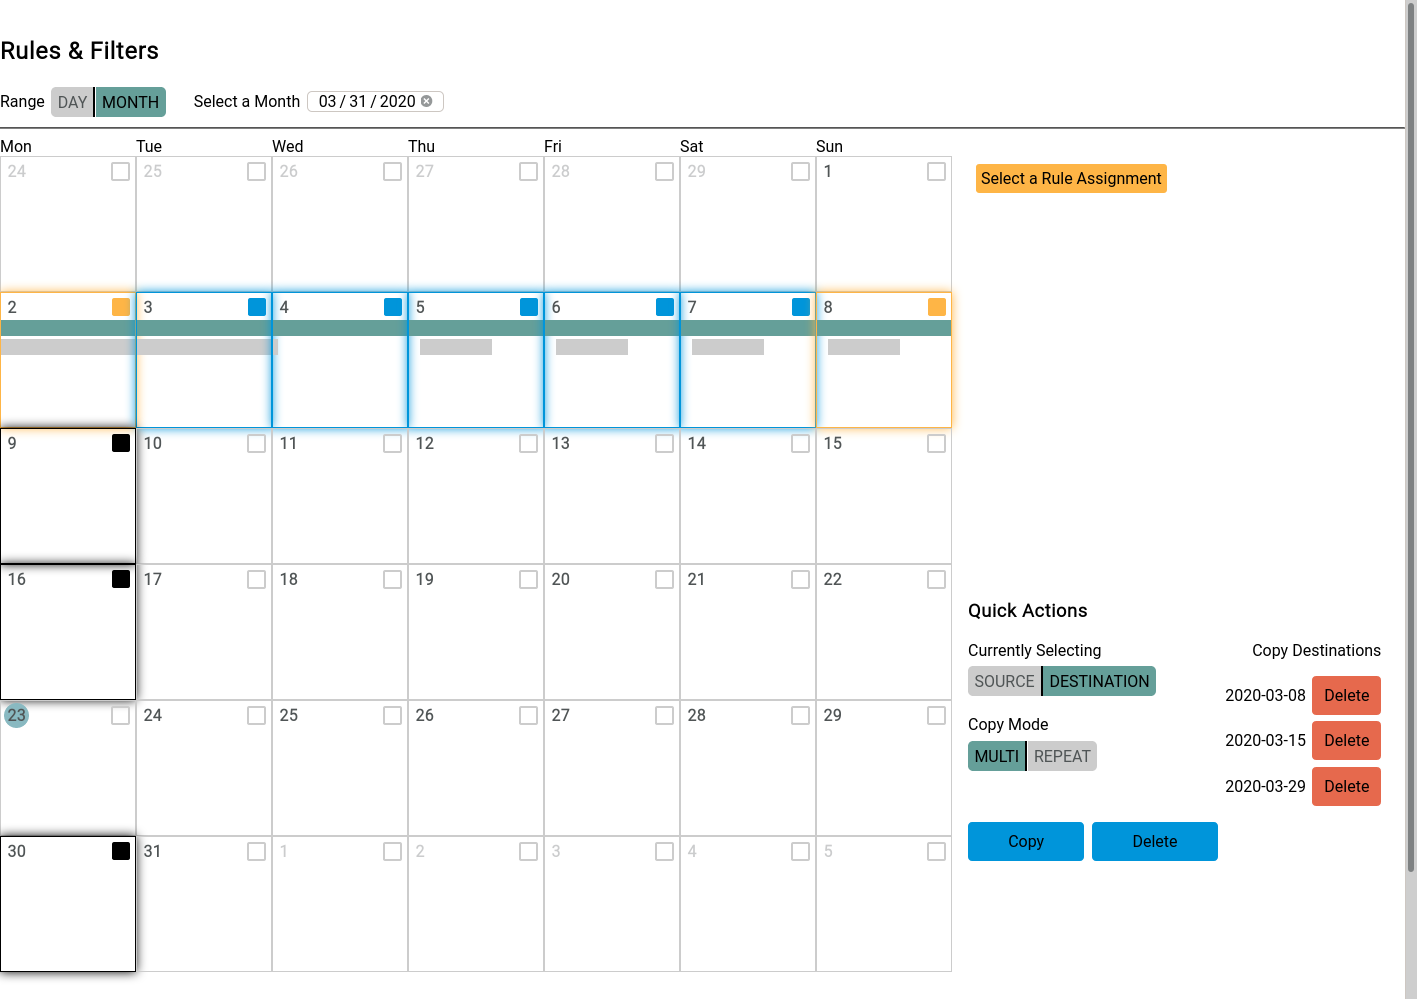
\includegraphics[width=145mm]{../img/page_rules_filters2.png}
  \caption[Stránka s pravidly a filtry -- pohled na jeden měsíc.]{Stránka s pravidly a filtry -- pohled na jeden měsíc.
  Kliknutí na tlačítko \textit{Copy} by zkopírovalo přiřazení pravidel mezi žlutě označenými dny na černě označené dny.
  Výsledek zkopírování je na následujícím obrázku.}
  \label{fig:page_rules_filters2}
\end{figure}

\begin{figure}[htb!] \centering
  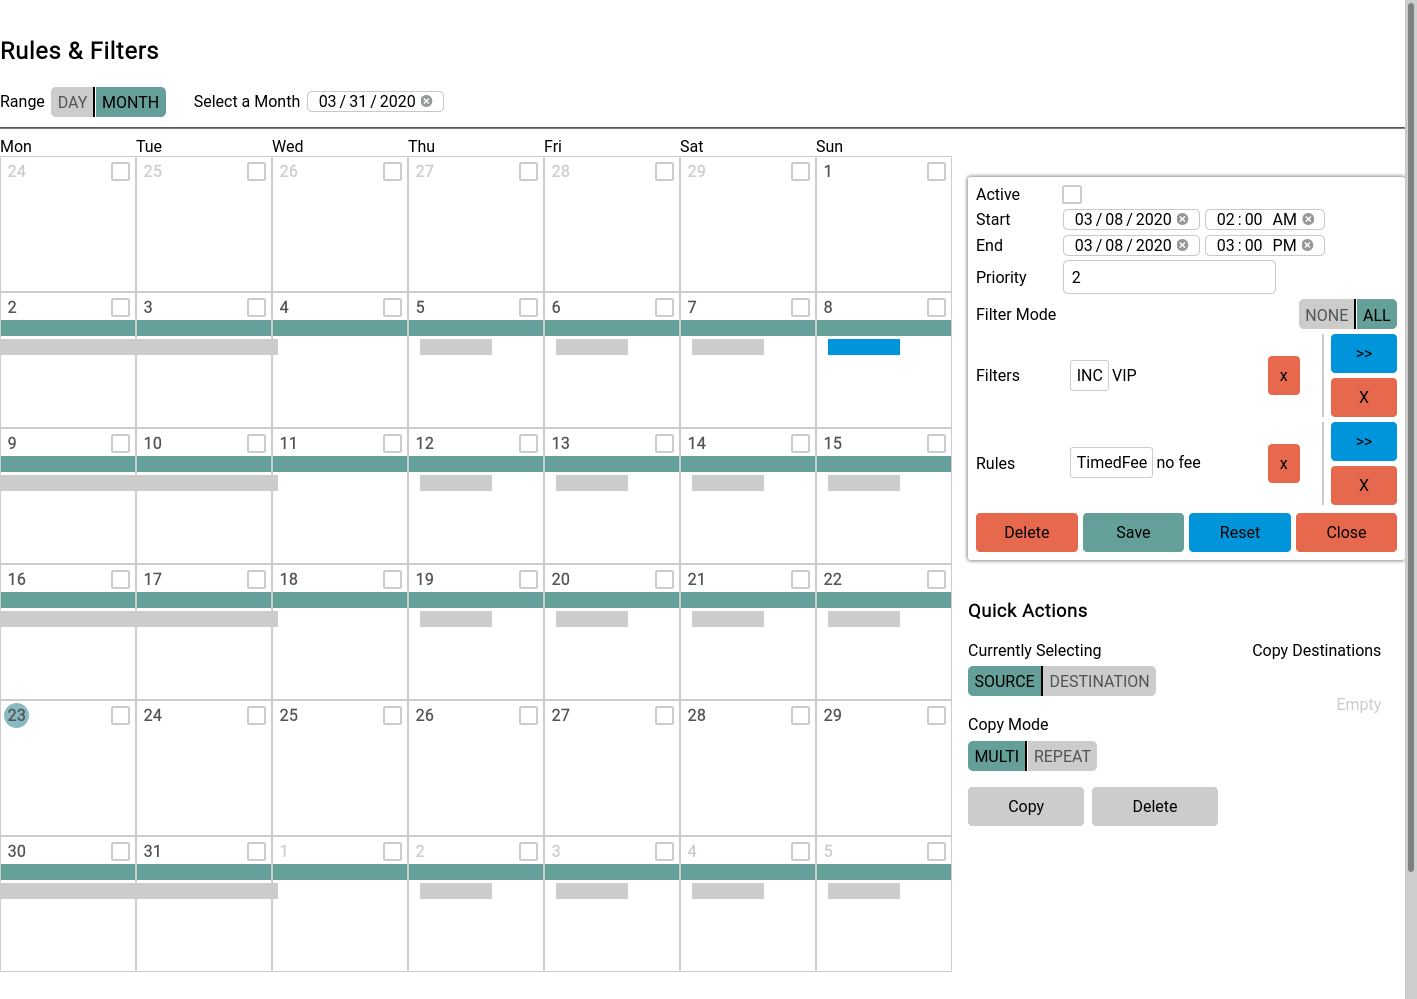
\includegraphics[width=145mm]{../img/page_rules_filters3.png}
  \caption[Stránka s pravidly a filtry -- výsledek kopírování.]{Stránka s pravidly a filtry -- výsledek kopírování.
  Vpravo nahoře lze navíc editovat zvolené přiřazení pravidel.}
  \label{fig:page_rules_filters3}
\end{figure}

\subsection{Vozidla a Parkování}

\noindent
Na této stránce lze zobrazit záznamy parkování, které obsahují čas vjezdu a výjezdu,
aplikovaná pravidla, vypočítanou částku k zaplacení pro konkrétní záznam a také vozidla,
kdy parkovala a kolik bylo celkem naúčtováno jednomu vozidlu.

Screenshoty obrazovky jsou na obrázcích \ref{fig:page_vehicles1} a \ref{fig:page_vehicles2}.

\begin{figure}[htb!] \centering
  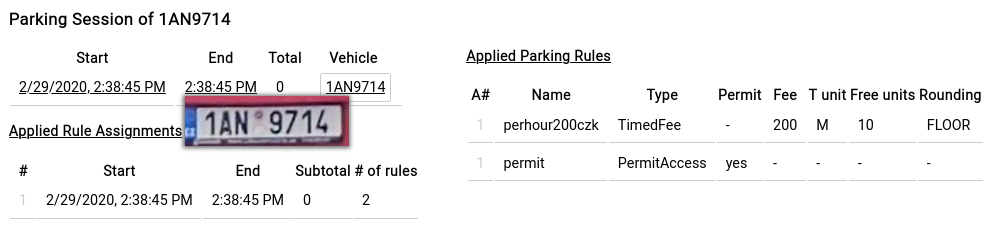
\includegraphics[width=145mm]{../img/page_vehicles1.png}
  \caption[Stránka se záznamy parkování.]{Stránka se záznamy parkování. V levém horním kvadrantu
  se nachází záznam parkování. Při najetí myši na čas vjezdu/výjezdu se zobrazí výřez rozpoznané SPZ.
  Navíc lze zkontrolovat použitá pravidla.
  Zároveň lze kliknout na SPZ a zobrazit si ostatní záznamy onoho vozidla na stejné obrazovce.
  Vpravo lze vidět vybírátka záznamů a vozidel. V levém dolním kvadrantu je pak detail jednoho
  vozidla.}
  \label{fig:page_vehicles1}
\end{figure}

\begin{figure}[htb!] \centering
  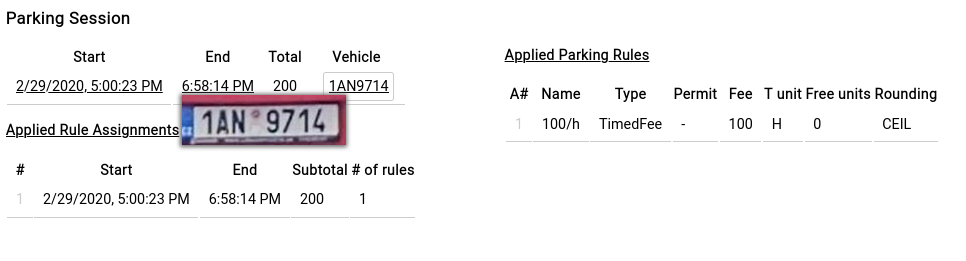
\includegraphics[width=145mm]{../img/page_vehicles2.png}
  \caption[Záznam parkování.]{Záznam parkování s výřezem naskenované SPZ.}
  \label{fig:page_vehicles2}
\end{figure}

\subsection{Statistiky}

\noindent
Tato stránka detailně zobrazuje údaje o počtu parkování a výdělku podle roku, měsíce a dne s grafy.
Zároveň zobrazuje počet vozidel na parkovišti.
Jeden z grafů je zobrazen na obrázku \ref{fig:google_charts} v podpodkapitole \ref{graphs}.

\newpage

\section{Autentizace a autorizace} \label{auther_authen}

\noindent
Autentifikace lidských uživatelů probíhá pomocí standardního hesla a autentifikace zařízení pomocí dlouhého,
náhodně generovaného hesla,
které je posíláno na frontend ve formě QR kódu, které zařízení naskenuje.
Po úspěšné autentizaci obdrží klient token.
Kdyby klient posílal token v souboru Cookie, vystavoval by se riziku útoku CSRF/XSRF.
Místo toho bude klient posílat token v hlavičce \textit{Authorization}.

Podle tokenu je klient jednoznačně identifikovatelný. Endpointy a GraphQL resolvery jsou zabezpečeny tak,
že každý endpoint nebo resolver, jenž vyžaduje oprávnění, dáme jako argument HOF (abbrv. Higher-Order-Function)
\textit{checkPermissions} společně s požadovanými oprávněními. \textit{checkPermissions} pak zavolá původní
endpoint nebo resolver, pouze pokud má klient dostatečná oprávnění.

\section{Komunikace}

\subsection{Endpointy backendu} \label{endpoints}

\noindent
Backend má pouze několik endpointů. Pro komunikaci s webovým rozhraním přes GraphQL.
Mobilní zařízení GraphQL nevyužívají, protože GraphQL není k nahrávání snímků vhodné a míchání více způsobů
komunikace pro velice malou mobilní aplikaci by vývoj spíše ztížilo. Máme tedy další endpointy:

\begin{itemize}
  \setlength\itemsep{.05em}
  \item POST \textit{/graphql} je určen k primární komunikaci s webovým rozhraním včetně autentifikace.
  \item GET \textit{/devices/qr/:id} slouží k získání QR kódu ve formě PNG obrázku z webového rozhraní pro autentifikaci zařízení.
        Přijímá \textit{id} zařízení jako parametr v URL.
  \item POST \textit{/devices/activate} slouží k autentifikaci zařízení, které právě naskenovalo QR kód s aktivačním heslem, které je posláno v těle žádosti.
  \item PUT \textit{/devices/config} slouží zařízení k získání své konfigurace a případné změně konfigurace ze strany zařízení.
  \item POST \textit{/devices/capture} přijímá obrazová data od zařízení.
  \item GET \textit{/captureImage/:id} slouží k získání výřezu naskenované SPZ z webového rozhraní. Přijímá \textit{id} obrázku jako parametr v URL.
\end{itemize}

\subsection{GraphQL resolvery}

\noindent
Protože GraphQL je primárním způsobem komunikace mezi frontendem a backendem, stojí za to si vysvětlit základní stavební bloky
GraphQL -- resolvery, které tvoří strom. Vzpoměňme si na příklad z předchozí kapitoly na obrázku \ref{fig:graphql_example}.
Zde kořenem stromu je resolver \textit{userSearch}, jenž přijímá argumenty potřebné pro jeho běh, ty jsou v tomto případě
povinné (ale nemusí). Kořenový resolver je funkce vracející nějaký typ, v tomto případě typ \textit{UserSearchResult}, který udává nalezené
uživatele (\textit{UserSearchResult.data}) a stránkování (v příkladu vynecháno).
Při návrhu tohoto resolveru bychom si mohli rozmyslet, že údaje o stránkování vynecháme a vrátíme pouze
pole neprázdných uživatelů -- typ \textit{[User!]}.
Máme dva druhy typů: skaláry (listy stromu) a objekty (uzly stromu).
Typ \textit{User} je objekt a má v sobě také nějaké hodnoty a vrátí se nám jen ty, na které se zeptáme. Měl-li by typ \textit{User}
další objekty, mohli bychom se zeptat i na jejich hodnoty. Kdybychom psali aplikaci pro veterinární kliniku, mohli bychom se zeptat
třeba na jména mazlíčků.

Jak toto implementujeme? Pro každý kořenový resolver musíme napsat funkci, která buď přímo vrátí požadovaný objekt s atributy, a nebo
k typu, který náš kořenový resolver vrací, napíšeme další resolvery, které vrací opět objekty, nebo skaláry.
Kdybychom se databáze ptali na uživatele i s
mazlíčky (v SQL terminologii bychom provedli JOIN), tak bychom nemuseli pro typ \textit{User} psát resolver pro mazlíčky, kde bychom
se dotázali na mazlíčky našeho uživatele.
\citep[][]{GraphQLDoc}

Zároveň můžeme provádět virtualizaci atributů -- přidávat atributy, které v databázi nemáme, ale pro webové rozhraní se hodí.
Hypotetickým příkladem budiž celková zaplacená částka zákazníkem, která se v případě potřeby vypočítá nebo aktuální agregované statistiky.
\subsection{Obecné resolvery}

\noindent
Jelikož se většina operací nad modely opakuje, byly napsány obecné resolvery jako HOF (abbrv. Higher-Order-Function)
pro vytváření, úpravu, mazání, vyhledávání a získávání modelů v relaci.
Měnící se část je pak pouze definice databázového modelu. Díky GraphQL se neumísi ani ověřovat datové typy --
GraphQL toto udělá podle schema, které tvoří programátor v SDL (abbrv. Schema-Definition-Language).
Na obrázku \ref{fig:generic_resolver} lze vidět funkci vracející resolver, který vrátí objekt v relaci
(provede JOIN v SQL terminologii), pokud ho vlastnící objekt ještě nemá.

\begin{figure}[!htb]
\lstset{language=Javascript}
\begin{lstlisting}
function gqlPopulate<D extends mongoose.Document,
                     K extends keyof D>(
  modelGetter: ModelGetter<D>,
  key: K
): Resolver {
  return async function(obj: D, args, ctx: Context, info) {
    // Get the model
    const model = modelGetter(ctx);
    const keyStr = key.toString();
    if (obj.populated(keyStr)) {
      // Already populated
      return obj[key];
    } else {
      // Fetch the field K on D only
      const populated: D = await model.populate(obj, {
        path: keyStr
      });
      // Resolver returns just the field K
      return populated[key];
    }
  };
}
\end{lstlisting}
% \centering
\caption[Ukázka obecného resolveru v Typescriptu.]{Ukázka obecného resolveru v Typescriptu. Na osmém řádku se získá model z funkce v \textit{lexical-scope} funkce vracející resolver. Proměnná \textit{ctx} definuje kontext resolveru a obsahuje modely a klienta, aby bylo snažší resolvery testovat -- jedná se o \textit{dependency injection}. Na šestém řádku lze vidět parametry, které dostává každý resolver. První parametr je objekt vrácený nadřazeným resolverem. Druhý parametr obsahuje klientem specifikované argumenty, například $id$ hledaného uživatele. Třetí parametr je již zmíněný kontext, jeho obsah si lze definovat dle libosti. Poslední parametr obsahuje informace o dotazu samotném -- jaké parametry si klient vyžádal, AST (angl. Abstract-Syntax-Tree) dotazu apod.}
\label{fig:generic_resolver}
\end{figure}

\subsection{Tvorba Apollo klienta}

\noindent
Webové rozhraní komunikující s backendem využívá již zmíněnou klientskou verzi knihovny Apollo, aby si vytvořila klienta,
který má mnoho paremetrů.

Nejdůležitější z nich jsou funkce, které řeší zpracování žádosti i odpovědi, jimž se říká \textit{links}.
Ty řeší zpracování chyb a poslání chyb do Reduxu, přečtení URL backendu z nastavení, také vložení tokenu do hlavičky žádosti ( \ref{auther_authen}).
Jejich způsob použití lze přirovnat k návrhovému vzoru \textit{chain-of-responsibility}.

Další parametr je určen ke cachování a vložení GraphQL schema získaného z backendu, aby bylo možné používat v dotazech fragmenty.

\subsection{Získávání obrázků}

\noindent
Jelikož se k autorizaci používá header \textit{Authorization} místo souborů cookies,
způsob získávání obrázků z endpointů zmíněných v \ref{endpoints} není obvyklý.
Namísto nastavení atributu \textit{src} HTML tagu \textit{img} na normální URL obrázku,
použijeme Blob URL. Obrázek stáhneme v Javascriptu a vytvoříme Blob URL pomocí API prohlížeče.
Přibližná implementace je ukázána na obrázku \ref{fig:image_getter}.

\begin{figure}[!htb]
\lstset{language=Javascript}
\begin{lstlisting}
function imageGetter(url: string): Promise<Response> {
  const url = `${config.backendApi.root}/${url}`;
  return fetch(url, {
    method: "GET",
    headers: {
      Authorization: `Bearer ${localStorage.getItem("token")}`
    }
  });
};

// In a component, setBlobUrl and setError are React hooks
function blobImage(url: string, setBlobUrl: string => void,
                   setError: any => void) {
  imageGetter(url)
    .then(response => response.blob())
    .then(blob => {
      setBlobUrl(URL.createObjectURL(blob));
    })
    .catch(setError);
}
\end{lstlisting}
\caption{Získání obrázků za použití hlavičky \textit{Authorization} a jejich zpracování.}
\label{fig:image_getter}
\end{figure}

\section{Ukládání a mazaní výřezů SPZ}

\noindent
Pokud je rozpoznána SPZ, nalezená SPZ se z obrázku vyřízne, a pak je dostupná k zobrazení ve webovém rozhraní.
% Tuto funkci lze vypnout ve webové aplikaci a zároveň lze výřezy smazat podle data vytvoření a
% lze nastavit automatické mazání po uplynuté době.
Výřezy jsou získány pomocí knihovny sharp a souřadnic SPZ od OpenALPR.
Zvolený způsob uložení je standardní dokument v MongoDB. Data jsou zakódována do base64,
a handler endpointu \textit{/capture-Image/:id} (viz podpodkapitola \ref{endpoints}) je dekóduje zpět.

První alternativou bylo využít GridFS MongoDB, ten je určen pro soubory
nad 16MB (limit formátu BSON) nebo pokud je potřeba číst jen části souborů. \citep{MongoDBGridFS}
Výřezy přibližně 500x100 pixelů jsou však mnohonásobně menší a vždy jsou načítány celé.
Druhou alternativou by byl souborový systém, ale mít všechna data v databázi je praktičtější.

\section{Parkovací pravidla} \label{analysis_parking_schema}

\noindent
Nechť umí parkovací pravidla následující:

\begin{itemize}
  \setlength\itemsep{.05em}
  \item Různá vozidla mohou podléhat různým pravidlům.
  \item Pravidla mají prioritu.
  \item Pravidla mají časové omezení.
  \item V jednu chvíli může platit více pravidel.
\end{itemize}

\noindent
Mechanismus, kterým umožníme vozidlům být ovlivněna některými pravidly,
budou filtry.
Pro jednoduchost je zapotřebí oddělit samotná pravidla od jejich
priority, časového intervalu platnosti i filtrů,
k čemuž bude sloužit objekt typu ParkingRuleAssignment.

\begin{figure}[!htb]
\lstset{language=GraphQL}
\begin{lstlisting}
type ParkingRuleAssignment {
  id: ID!
  rules: [ParkingRule]!
  start: DateTime!
  end: DateTime!
  vehicleFilterMode: VehicleFilterMode!
  vehicleFilters: [VehicleFilter!]
  priority: NonNegativeInt!
}

type VehicleFilter {
  id: ID!
  name: String!
  action: VehicleFilterAction!
  vehicles: [Vehicle!]
}
\end{lstlisting}
\caption[Definice typů ParkingRuleAssignment a VehicleFilter v GraphQL SDL.]{Definice typů ParkingRuleAssignment a VehicleFilter v GraphQL SDL.
Tučne jsou označeny rezervovaná slova a skáláry již obsažené v základním GraphQL.
Kurzívou jsou označeny skaláry z knihovny graphql-scalars.
Vykřičník značí, že atribut je povinný (nesmí být null v odpovědi).
Typ VehicleFilterMode je enum, jehož možné hodnoty jsou ALL, NONE.
Typ VehicleFilterAction je taktéž enum, jehož možné hodnoty jsou INCLUDE, EXCLUDE.}
\label{fig:type_pra_vf}
\end{figure}

Filtrování bude mít dva módy: začne se se všemi vozidly (ALL) a začne se bez vozidel (NONE).
Následné filtry mohou buď přidávat, nebo odstraňovat jednotlivá vozidla.
Hodí se mít filtry uložené separátně, aby mohly být využity několikrát.

\newpage
\subsection{Algoritmus filtru vozidel}

\noindent
\textit{Vstup: objekt ParkingRuleAssignment s filtry, vozidlo}

\noindent
\textit{Výstup: boolean určující zdali vozidlo prošlo filtrem}

\begin{enumerate}
  \setlength\itemsep{.05em}
  \item Na základě módu filtrování si budeme udržovat množinu buď odstraněných vozidel (mód ALL), nebo přidaných vozidel (mód NONE).
  \item Podle příslušné akce filtrů (odstranit nebo přidat) budeme manipulovat množinou vozidel.
        Např. je-li mód ALL a filtr odstraňuje, do množiny si vozidla přidáme, nebo pokud je-li mód NONE a filtr též odstraňuje, vozidla z množiny odstraňujeme.
  \item Pokud je vozidlo ve výsledné množině, tak pro něj ParkingRuleAssignment platí pokud je filtrovací mód NONE,
        ale neplatí pokud je mód ALL. Opačný výsledek se vrátí, pokud vozidlo v množině není.
\end{enumerate}

Časová i paměťová složitost algoritmu je ${\cal O}(N)$, kde $N$ je počet filtrů.
% Tento algoritmus lze potenciálně rozdělit na předvýpočet (kroky 1. a 2.) a ověření (krok 3.).
% Tato možnost zvýší paměťovou náročnost, protože bychom si museli pamatovat množiny, což je nepraktické.
% Je-li uživatel příčetný, počet použitých filtrů nebude obrovský, a tudíž je lepší zvolit následující způsob cachovaní.
% Zapamatujeme si výsledky pro určitý seznam filtrů pro konkrétní vozidlo pouze při běhu algoritmu, který je
% vysvětlen v následující podkapitole, čímž následující algoritmus zrychlíme.

\subsection{Algoritmus pro aplikaci pravidel}

\begin{figure}[!htb] \centering
  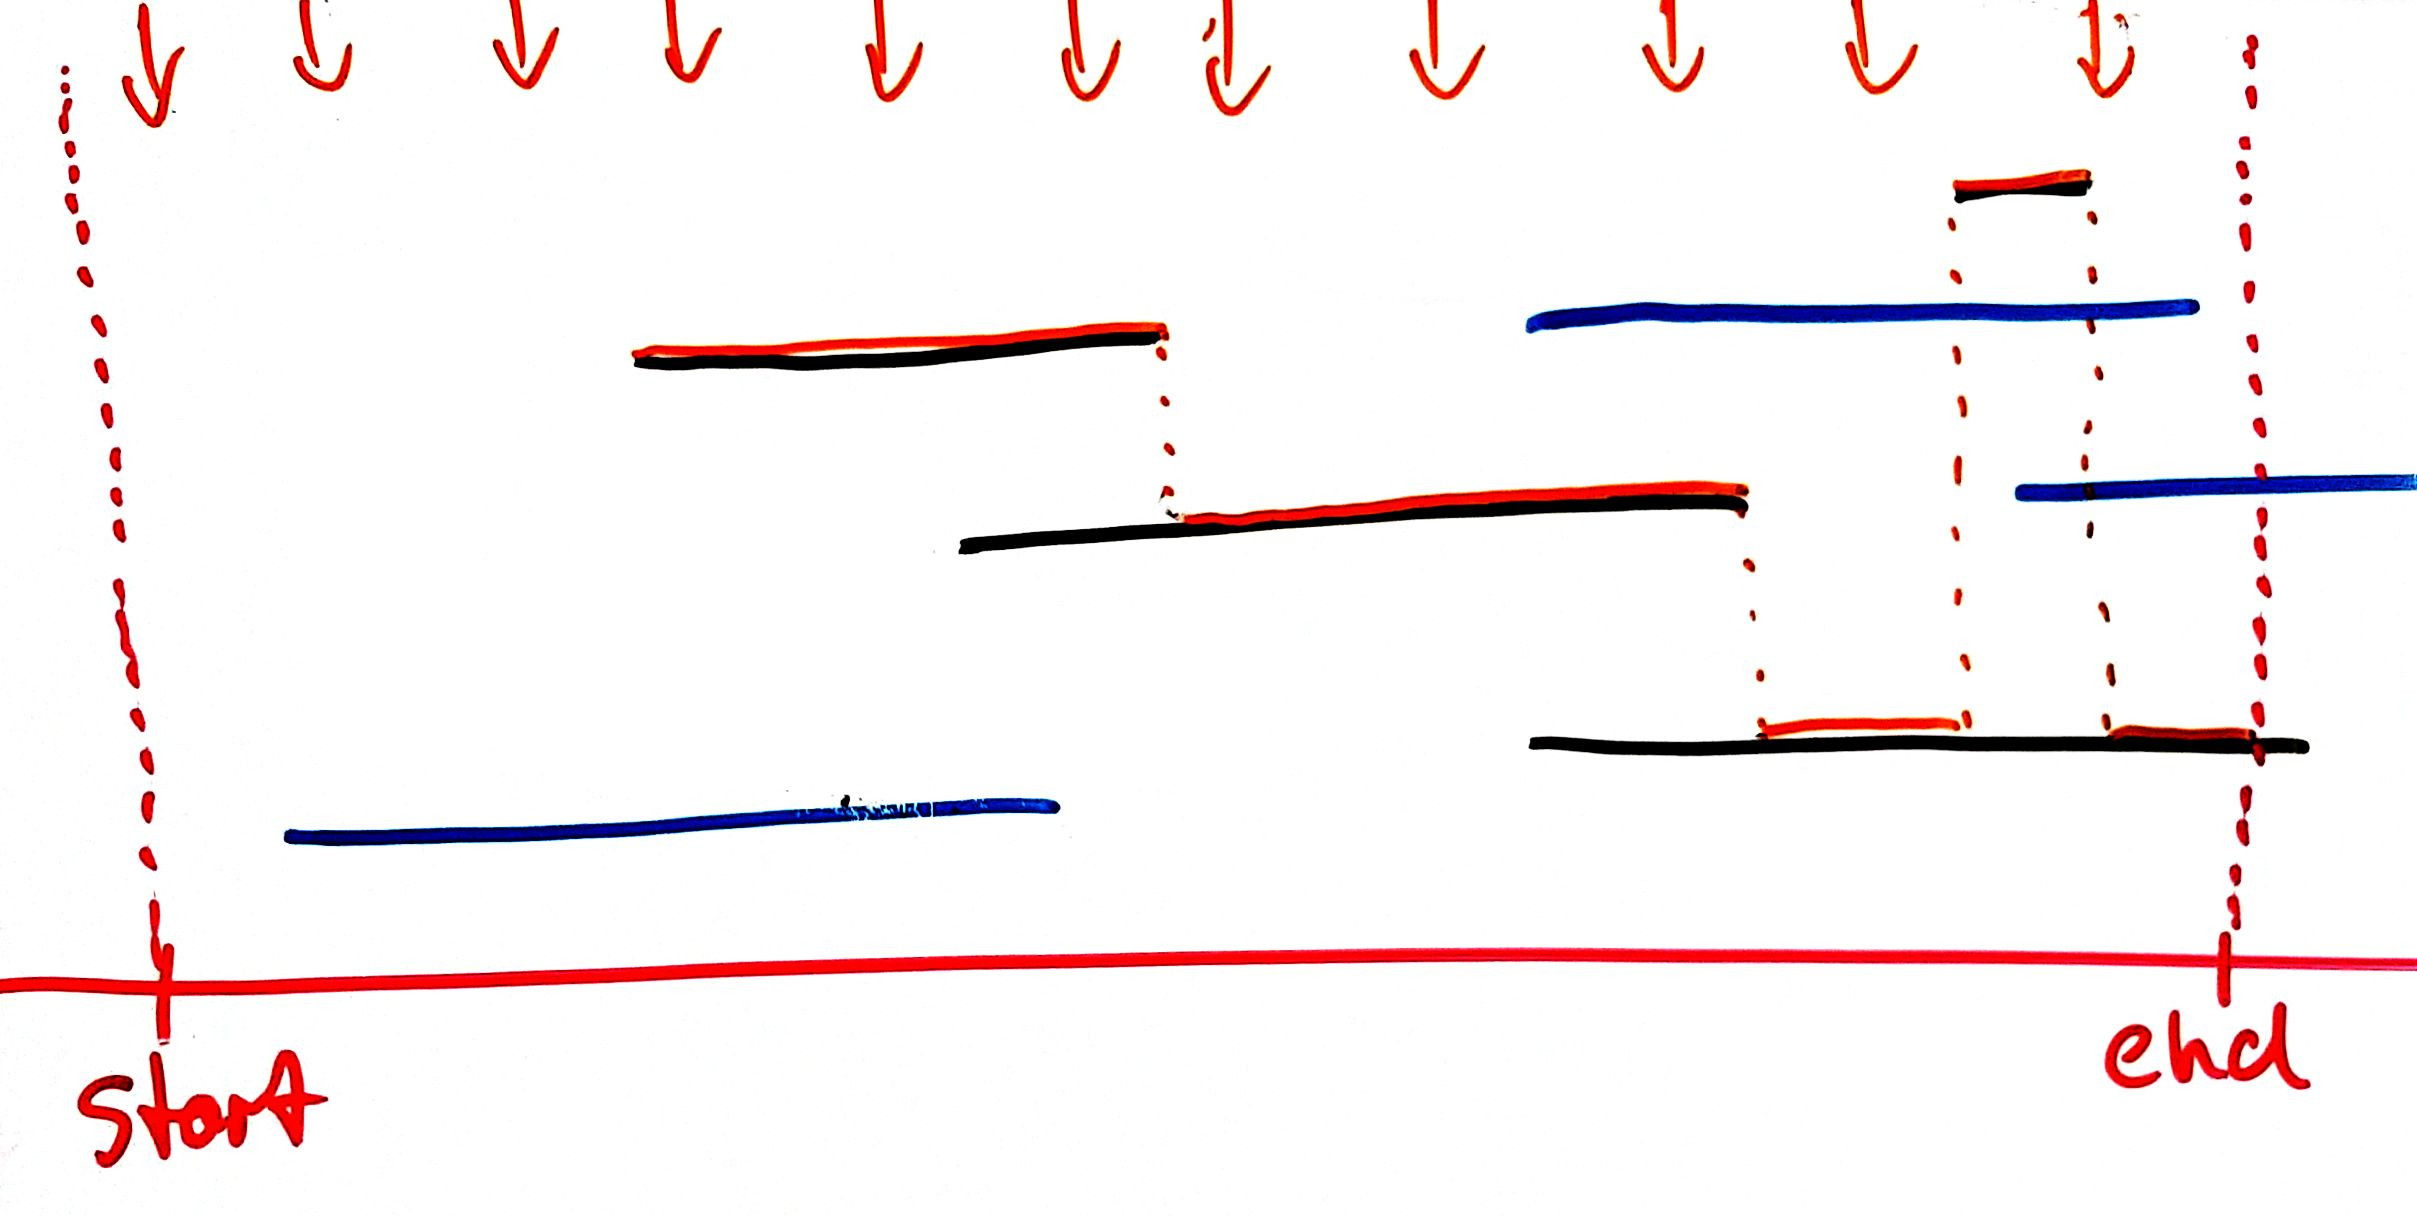
\includegraphics[width=145mm]{../img/rules_drawing.jpg}
  \textit{Modré úsečky neplatí kvůli filtrům nebo protože jsou deaktivované. Oranžová čára značí výstup požadovaného algoritmu.}
  \caption{Ilustrace problému úseček.}
  \label{fig:rules_drawing}
\end{figure}

\noindent
Pro zjednodušení algoritmu, uvalíme omezení: ve stejný čas nesmí existovat více ParkingRuleAssignment
se stejnou prioritou.

Situaci si lze představit jako několik navzájem rovnoběžných úseček v různých výškách, které se neprotínají.
Nás nyní zajímá, na které a v jakých intervalech na ně dopadne světlo, pokud na ně kolmo zeshora posvítíme.
Na obrázku \ref{fig:rules_drawing} je ilustrace tohoto geometrického problému.

Pro zjednodušení popisu algoritmu předpokládejme, že všechny ParkingRuleAssignment, které zpracováváme, platí pro naše vozidlo.
Přidat tuto kontrolu později je triviální.

\vspace{5mm}
\noindent
\textit{Vstup: seznam ParkingRuleAssignment platných v intervalu pobytu vozidla na parkovišti, vozidlo}

\noindent
\textit{Výstup: seznam ParkingRuleAssignment s časy platnosti}

\begin{enumerate}
  \setlength\itemsep{.05em}
  \item Seřadíme si začátky a konce úseček podle jejich času.
  \item Vytvoříme si haldu pro odkládání úseček, která řadí podle priority -- větší výše.
  \item Vytvoříme si seznam aplikovaných pravidel s časy (časy se mohou lišit od počátečních i koncových časů).
  \item Nechť \textit{s} je současná úsečka a \textit{$t_s$} čas zvolení \textit{s} (čas zvolení se může lišit od začátku úsečky).
  \item Pro každou událost \textit{u} značící začátek/konec úsečky (aplikaci pravidla) \textit{p}:
  \begin{enumerate}
    \item Pokud se jedná o začátek nové úsečky:
    \begin{enumerate}
      \item Pokud není zvolená úsečka:\\
            \textit{$t_s$} $\leftarrow$ \textit{p.start}\\
            \textit{s} $\leftarrow$ \textit{p}
      \item Pokud je zvolená úsečka a \textit{p} má vyšší prioritu než \textit{s}:\\
            \textit{s} dáme do seznamu aplikovaných pravidel se začátkem \textit{$t_s$} a koncem \textit{p.start}.\\
            \textit{s} dáme na haldu, pokud \textit{s.end} > \textit{p.end}.\\
            \textit{$t_s$} $\leftarrow$ \textit{p.start}\\
            \textit{s} $\leftarrow$ \textit{p}
      \item Pokud je zvolená úsečka a \textit{p} má nižší prioritu než \textit{s} a \textit{p.end} > \textit{s.end}:\\
            \textit{s} dáme na haldu
    \end{enumerate}
    \item Jinak (jedná se o konec nějaké úsečky):
    \begin{enumerate}
      \item Přidáme \textit{s} do seznamu aplikovaných pravidel se začátkem \textit{$t_s$} a koncem \textit{s.end}.
      \item Taháme z haldy, dokud nedostaneme úsečku s koncem později než koncem \textit{p}, nebo dokud halda není prázdná.
      \item Pokud jsme z haldy vhodnou úsečku vytáhli, použijeme ji. V opačném případě vyprázdníme \textit{s} a \textit{$t_s$}.
    \end{enumerate}
  \end{enumerate}
\end{enumerate}

\noindent
Algoritmus zajisté doběhne, protože máme konečný počet událostí a v každém cyklu jednu zpracujeme.
Paměťová složitost je zřejmě lineární. Časová složitost bez filtrování je ${\cal O}(N\cdot{logN})$, kde $N$ je 
počet úseček, protože
využijeme některého z rychlích řazení a protože použijeme binární haldu nebo lepší haldu. Počet operací nad haldou,
který by konečnou složitost mohl změnit, je naštestí lineární. Největší počet operací nad haldou dostaneme tak, že
každou přidanou úsečku umístíme tak, aby při zpracování jejího konce i začátku došlo k přidání a odebrání z haldy
Jedno z takovýchto uspořádání je například pyramida, popřípadě zikkurat.
Tedy s každou přidanou úsečkou se počet operací nad haldou zvýší maximálně o $2$, což je lineární vzhledem k počtu úseček.

Přidáme-li filtrování, tak v nejhorším případě budeme ověřovat platnost každé úsečky. Bude-li $M$ průměrný počet
filtrů, pak je časová složitost ${\cal O}(N\cdot{M})$. 
% Při rozumném počtu \texttt{ParkingRuleAssignment} v daném intervalu je algoritmus velice rychlý

\section{Uživatelské rozhraní}

\noindent
Jelikož autor neměl zkušenosti s vývojem webového uživatelského rozhraní, rozhodl se využít starter projekt
společnosti Crazy Factory GmbH, který pojí vybrané technologie dohromady a mandatuje projektu základní strukturu.
Navíc podporuje překlady, reportování chyb apod., což je obtížné vytvářet z ničeho. \citep[][]{CFProj}

\subsection{Redux a persistence stavu}

\noindent
Jak již bylo zmíněno v předchozí kapitole, uživatelské rozhraní používá Redux pro sdílení stavu mezi komponentami.
Stav v Reduxu je strom, jenž je upravován akcemi. Akce a současný stav je předán takzvaným \textit{reducers}, což jsou prosté funkce,
které vrátí stav nový. \citep[][]{ReduxCore} Prostost reducerů zajišťuje testovatelnost.

Jako příklad konkrétního využití budiž sdílení některých údajů mezi obrazovkami.
Například sdílení vozidla mezi stránkou s vozidly a stránkou s pravidly, schopnost seznamu se záznamy o parkování
zvolit vozidlo a mnoho dalších.

Některé komponenty jsou pak na stavu závislé a dojde k jejich překreslení, pokud se jimi čtený stav změní, což je též zařízeno
Reduxem. Jedná se vlastně o formu \textit{dependency-injection}. Stejným mechanismem jsou do komponent vkládány
funkce vytvářející akce a jiné vedlejší efekty, což dělá tyto komponenty snadno testovatelné.

K uložení stavu aplikace po zavření okna, použijeme knihovnu redux-persist, která poskytuje
HOF (abbrv. Higher-Order-Function), které dáme reducer, a ona změny, které způsobí, někam uloží. \citep[][]{reduxpersist}
V našem případě se jedná o \textit{localstorage}.

\subsection{Typy komponent}

\noindent
Níže je rozlišení komponent podle jejich interakce s ostatními a míry autonomie.
Jedná se o spektrum, ne o kategorie.

\begin{itemize}
  \setlength\itemsep{0.05em}
  \item \textbf{Bez vnitřního stavu} -- může se jednat o tlačítka, vstupy textu apod. Tyto komponenty jsou zcela řízeny
      nadřazenou komponentou. S nadřazenou komponentou komunikují pomocí callback funkcí, které komponenta přijímá jako parametry.
  \begin{itemize}
    \setlength\itemsep{0.05em}
    \item \textbf{Strukturní} -- delegují data dalším komponentám a mohou mít podřízené komponenty. Příkladem budiž sekce třeba v 
        uživatelském rozhraní se stejným stylem.
  \end{itemize}
  \item \textbf{S vnitřním stavem} -- tyto komponenty údávají stav podřízeným komponentám.
  \begin{itemize}
    \setlength\itemsep{0.05em}
    \item \textbf{Napojené na Redux} -- jedná se o podtyp komponent s vnitřním stavem, které část stavu berou z Reduxu.
    \item \textbf{Komunikující se světem} --  komunikují s vnějším světem. Například posílají GraphQL dotaz backendu.
  \end{itemize}
\end{itemize}

\subsection{Základní prvky uživatelského rozhraní}

\noindent
Každá složitější webová aplikace používá různé druhy tlačítek a vstupů.
Bohužel v každém prohlížeči vypadají základní prvky jinak. Na obrázku \ref{fig:browser_checkboxes}
je screenshot z webové stránky \url{https://developer.mozilla.org/en-US/docs/Web/HTML/Element/input/checkbox}.

Pokud se chce navíc uálně sjednotit tyto prvky se zbytkem uživatelského rozhraní, je
vyvinutí vlastních elementárních prvků nevyhnutelné. Vývoj se řídil principem minimu informací
-- omezí se v rámci jednoho prvku počet nápadných částí. V praxi to například znamená žádné nebo méně výrazné
 orámování (CSS vlastnost \textit{border}) a zahlé rohy (CSS vlastnost \textit{border-radius}).
Na obrázku \ref{fig:ui_elems} lze vidět prvky využité v projektu.

\begin{figure}[!htb] \centering
  
\includegraphics[width=70mm]{../img/chrome_checkbox.png}
  
\includegraphics[width=70mm]{../img/firefox_checkbox.png}
  \caption{Checkboxy v Mozilla Firefox a Google Chrome.}
  \label{fig:browser_checkboxes}
\end{figure}

\begin{figure}[htb!]
  \centering
  \begin{tabular}{@{}c@{}}
    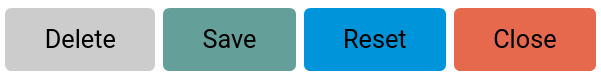
\includegraphics[width=70mm]{../img/buttons.png} \\
    \small (1) Tlačítka -- Delete je vypnut/disabled.
  \end{tabular}

  \vspace{\floatsep}

  \begin{tabular}{@{}c@{}}
    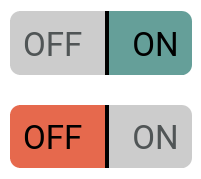
\includegraphics[width=24mm]{../img/two_pickers.png} \\
    \small (2) Přepínač -- zapnut a vypnut.
  \end{tabular}

  \vspace{\floatsep}
  \begin{tabular}{@{}c@{}}
    
\includegraphics[width=28mm]{../img/checkboxes.png} \\
    \small (3) Checkbox ve stádiích vypnutí, přejíždění myší, zapnutí a opět přejíždění myší.
  \end{tabular}

  \vspace{\floatsep}
  \begin{tabular}{@{}c@{}}
    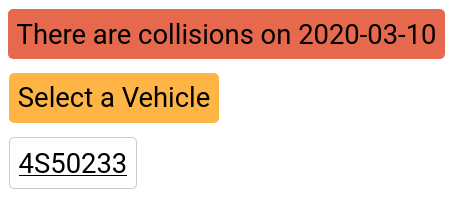
\includegraphics[width=70mm]{../img/ui_flag.png} \\
    \small (4) Zvýrazňovač -- chyba, upozornění a SPZ (podtržení značí interaktivnost).
  \end{tabular}
  \caption{Základní prvky uživatelského rozhraní.}
  \label{fig:ui_elems}
\end{figure}


\subsection{Grafy} \label{graphs}

\noindent
Grafy jsou potřeba na stránce se statistikami. K tomu byla použita knihovna react-google-charts,
což, jak název napovídá, je port knihovny google-charts do Reactu. Ta kromě obvyklích grafů umí
například i takzvaný kalendářový graf, jenž lze vidět na obrázku \ref{fig:google_charts}.

\begin{figure}[!htb] \centering
  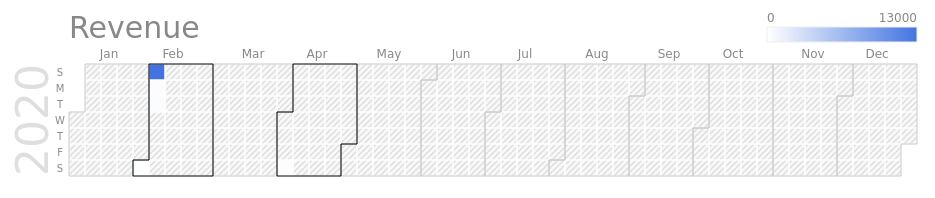
\includegraphics[width=145mm]{../img/google_charts.png}
  \caption{Kalendářový graf z knihovny react-google-charts.}
  \label{fig:google_charts}
\end{figure}

\subsection{Obecná vybírátka modelů}

\noindent
Dle principu neopakování se bylo vytvořeno několik obecných UI komponent, které umožňují vyhledávání libovolných
modelů a jejich volbu a využití v ostatních komponentách. Ve zdrojovém kódu je implementujeme jako
HOF (aabrv. Higher-Order-Function), což je funkce vracející další funkce -- konkrétní komponenty.
Měnící se části, které se do těchto obecných komponent budou vkládat, je komponenta renderující jediný model
(\textit{renderModel}),
GraphQL dotaz pro získávání modelů (\textit{queryString}), funkce, jejímž vstupem je odpověď na GraphQL dotaz a výstupem je
samotné pole modelů (\textit{modelArrayGetter}), a funkce, jejímž vstupem je dotazovací řetězec a výstupem jsou
argumenty pro GraphQL dotaz (\textit{identifierToOptions}).

Obrázek \ref{fig:picker_lifecycle} ukazuje tok dat v jednom z obecných vybírátek.
Obrázek \ref{fig:picker_component} ukazuje vyrenderovanou komponentu vybírátka.

Další vybírátka abstrahují i vstup od uživatele, takže lze použít například kalendář.

\begin{figure}[!htb] \centering
  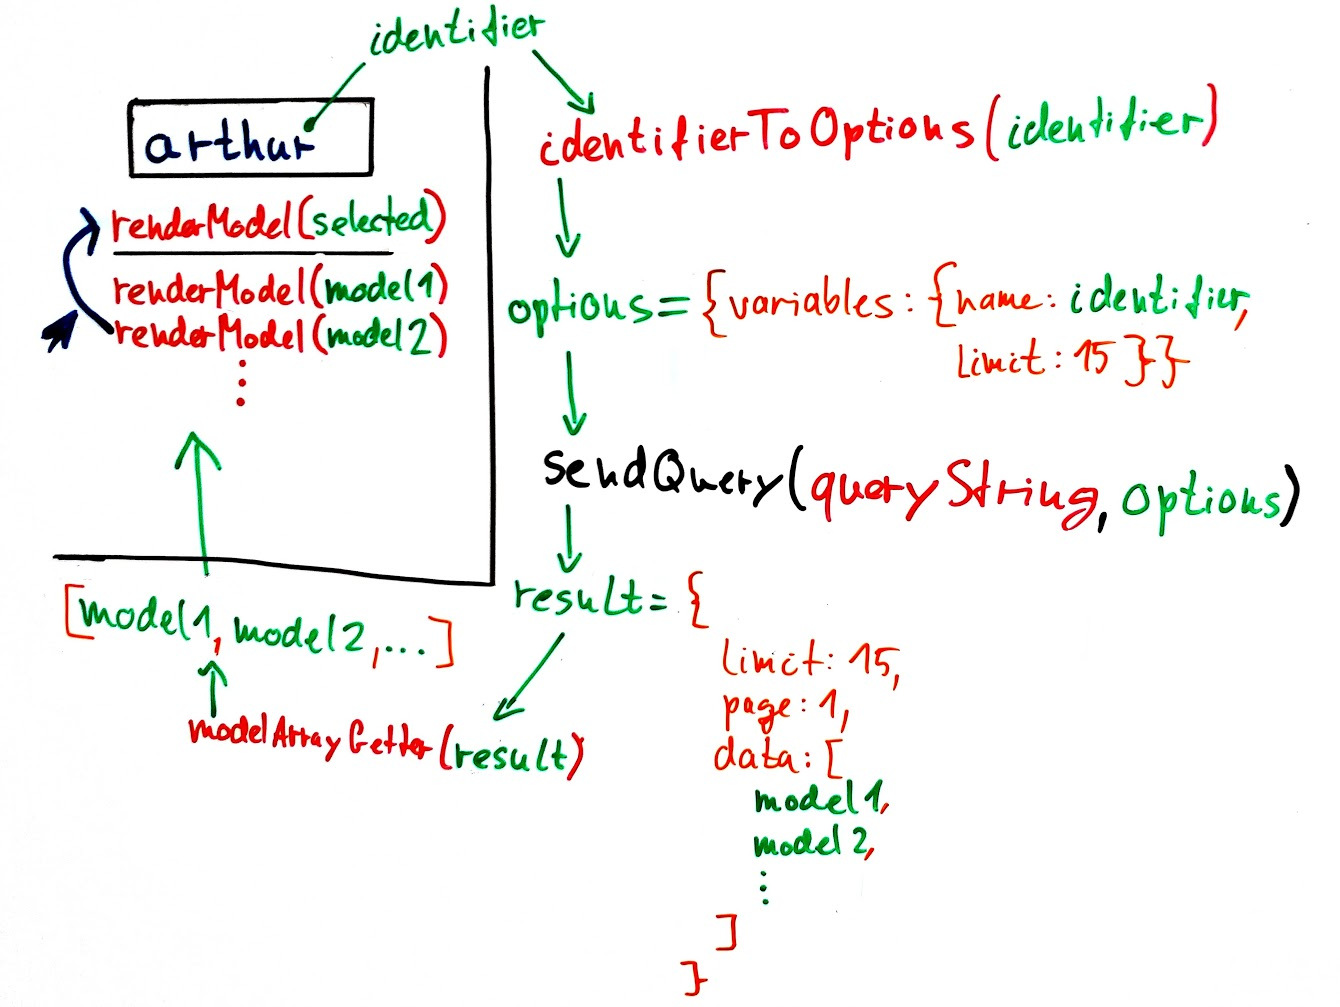
\includegraphics[width=145mm]{../img/picker_lifecycle.jpg}
  \caption{Tok dat v jednom z obecných vybírátek.}
  \label{fig:picker_lifecycle}
\end{figure}

\begin{figure}[!htb] \centering
  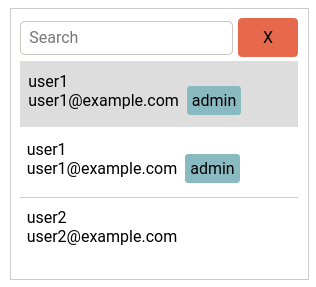
\includegraphics[width=70mm]{../img/picker_component.png}
  \caption[Vyrenderovaná komponenta jednoho vybírátka.]{Vyrenderovaná komponenta jednoho vybírátka. Šedivě podbarvený uživatel je zvolený.
  Při psaní do textového se ihned vyhledává hledaný objekt -- v tomto případě uživatel.}
  \label{fig:picker_component}
\end{figure}
